\title{Human Computer Interaction Terrestrial Globe}
\author{
        Alber S\'anchez, Jim Jones\\
        alber.sanchez@uni-muenster.de, jim.jones@uni-muenster.de\\        
        Institut f\"ur Geoinformatik\\
        Westf\"alische Wilhelms-Universit\"at, M\"unster, Deutschland\\
        \\
		- Physical Computing Final Report - 
        }
\date{\today}

\documentclass[12pt]{article}

\usepackage[top=2.5cm, bottom=2.5cm, left=4.5cm, right=3.5cm]{geometry}
\usepackage{listings}
\usepackage{epsfig}
\usepackage{url}
\usepackage{wrapfig}
%\usepackage[bookmarks=true,pdfborder={0 0 0},plainpages=false,pdfpagelabels]{hyperref}
\usepackage{mdwlist}
\usepackage{graphics}
\usepackage{listings}
\usepackage{color}
\usepackage{float}
\usepackage{eurosym}
\usepackage{verbatim}

%----------------------
%To support EPS graphics in TEXMAKER
%\usepackage{epstopdf}
%----------------------


\newenvironment{smallverbatim}{\endgraf\small\verbatim}{\endverbatim} 
\lstset{
         basicstyle=\footnotesize\ttfamily, % Standardschrift
         numbers=left,               % Ort der Zeilennummern
         numberstyle=\footnotesize,          % Stil der Zeilennummern
         %stepnumber=2,               % Abstand zwischen den Zeilennummern
         numbersep=5pt,              % Abstand der Nummern zum Text
         tabsize=2,                  % Groesse von Tabs
         extendedchars=true,         %
         breaklines=true,            % Zeilen werden Umgebrochen
         keywordstyle=\color{red},
    	 frame=tb,         
         stringstyle=\color{black}\ttfamily, % Farbe der String
         showspaces=false,           % Leerzeichen anzeigen ?
         showtabs=false,             % Tabs anzeigen ?
         xleftmargin=17pt,
         framexleftmargin=17pt,
         framexrightmargin=5pt,
         framexbottommargin=4pt,
         showstringspaces=false      % Leerzeichen in Strings anzeigen ?        
 }

\begin{document}
\maketitle

\paragraph{Keywords:}
HCI, Arduino, globe, Google-Earth, Processing.

\section{Outline}

This report aims to provide essential information about how the HCI Terrestrial Globe was built, from its inception to its final implementation, regarding the most important project milestones. In the section \textit{Project Overview} we will discuss the initial ideas, issues and solutions adopted for the project development. In the section \textit{Technologies Used} we go through the solution's architecture, explaining the importance and function of each project layer. Furthermore, in the section \textit{Arduino Embedded Software}, we describe in more detail the most important points about Arduino embedded code, libraries used and its main functions. Finally, in the section \textit{Processing Software}, we go through important aspects of the PC listener developed to control Google-Earth.

\section{Project Overview}

The HCI Terrestrial Globe was conceptualized by the search of a more intuitive and innovative way of controlling Google-Earth, based on a \EUR{50,00} budget. Based on this premise, we came up with the idea of controlling Google-Earth simply by rotating an sphere, giving users the feeling of rotating Google-Earth globe with their own hands. To achieve this, we decided to use a low cost solution for acquiring the sphere's two axis movements, namely two mouse sensors placed in the measured axis, which can provide the distance moved on each direction. In Figure \ref{fig:mouse1} you can see how the connection with the sensor (ADNS-2610\footnote{\url{http://www.avagotech.com/docs/AV02-1184EN}}) was made, connecting four cables between the Arduino board and the sensor, namely clock, data, power(5 volts) and ground. 
\\
\begin{figure}[h]\centering
%\includegraphics[scale=0.10]{mouse_sensor.eps} 
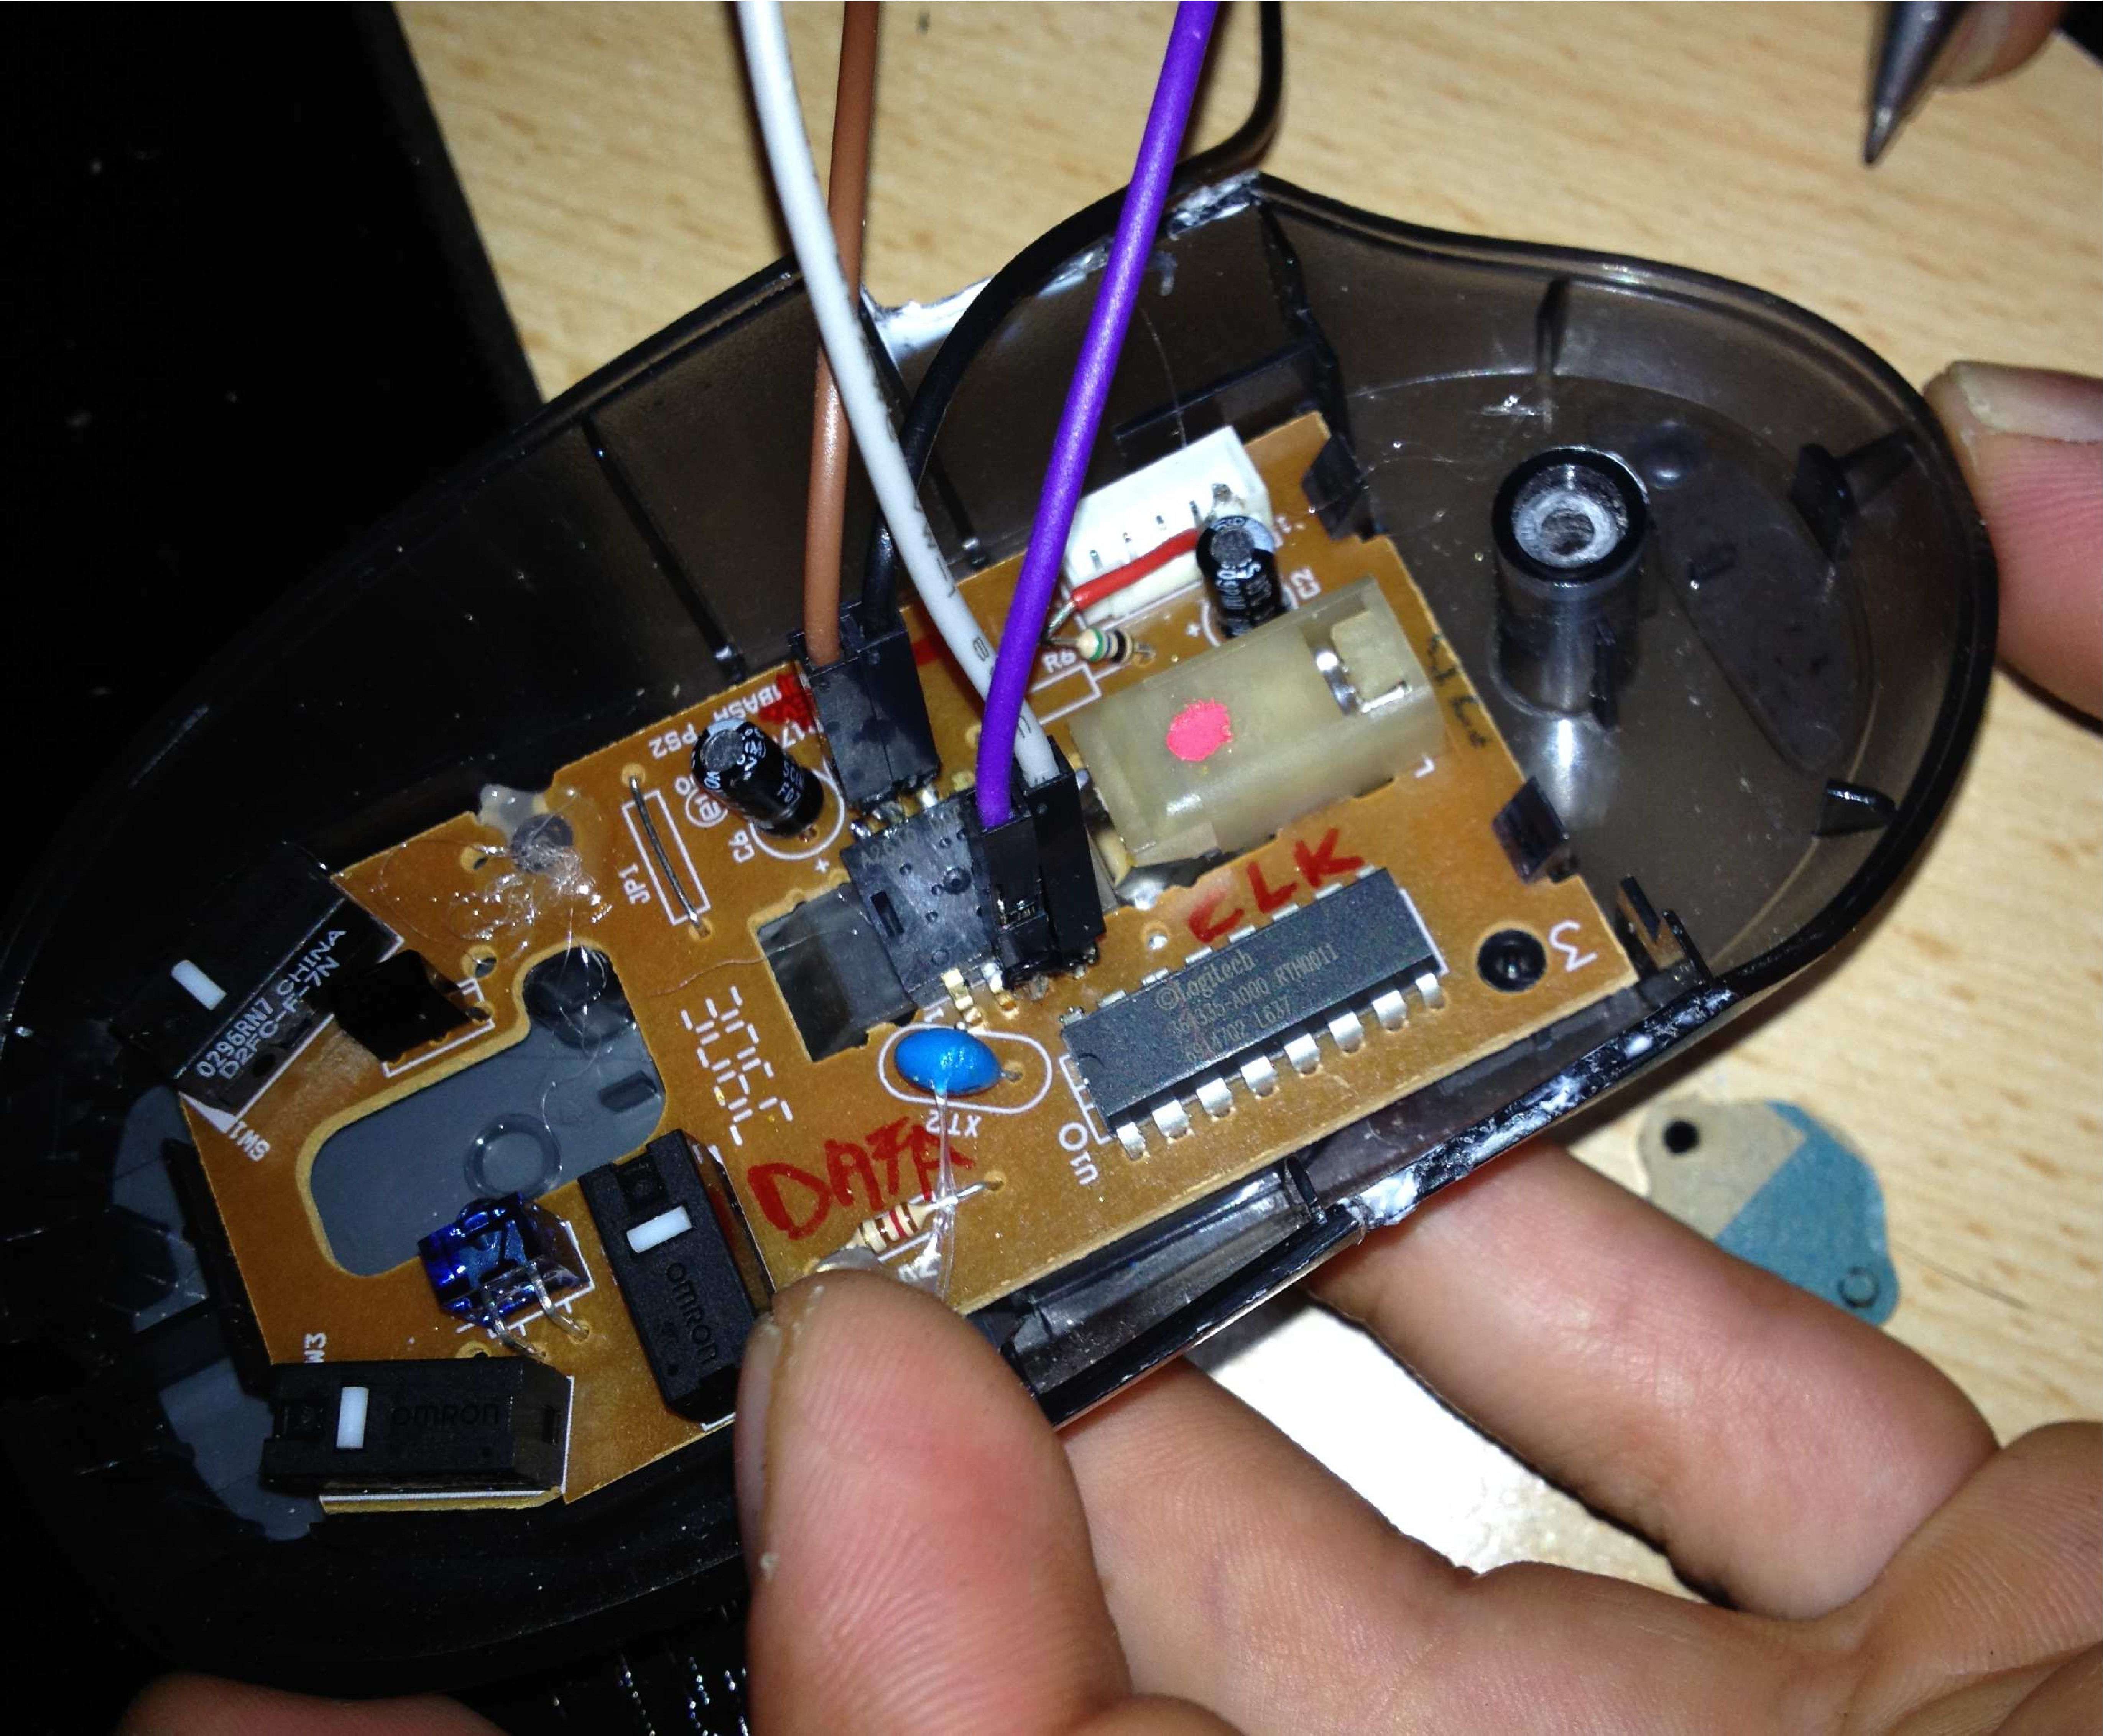
\includegraphics[scale=0.10]{mouse_sensor-eps-converted-to.pdf} 
\caption{Cables conneting to the mouse sensor}\centering 
\label{fig:mouse1}
\end{figure}	

After properly connecting the sensors to the Arduino board, a wooden case was built for holding the two mice, where the vertical mouse measures movements along the rolling sphere's Z and X axes and the other mouse along the Y axis. A first prototype of the case can be seen in the Figure \ref{fig:prot1} and Figure \ref{fig:prot2}.

\begin{figure}[h!]\centering
%\includegraphics[scale=0.10]{prototype1.eps} 
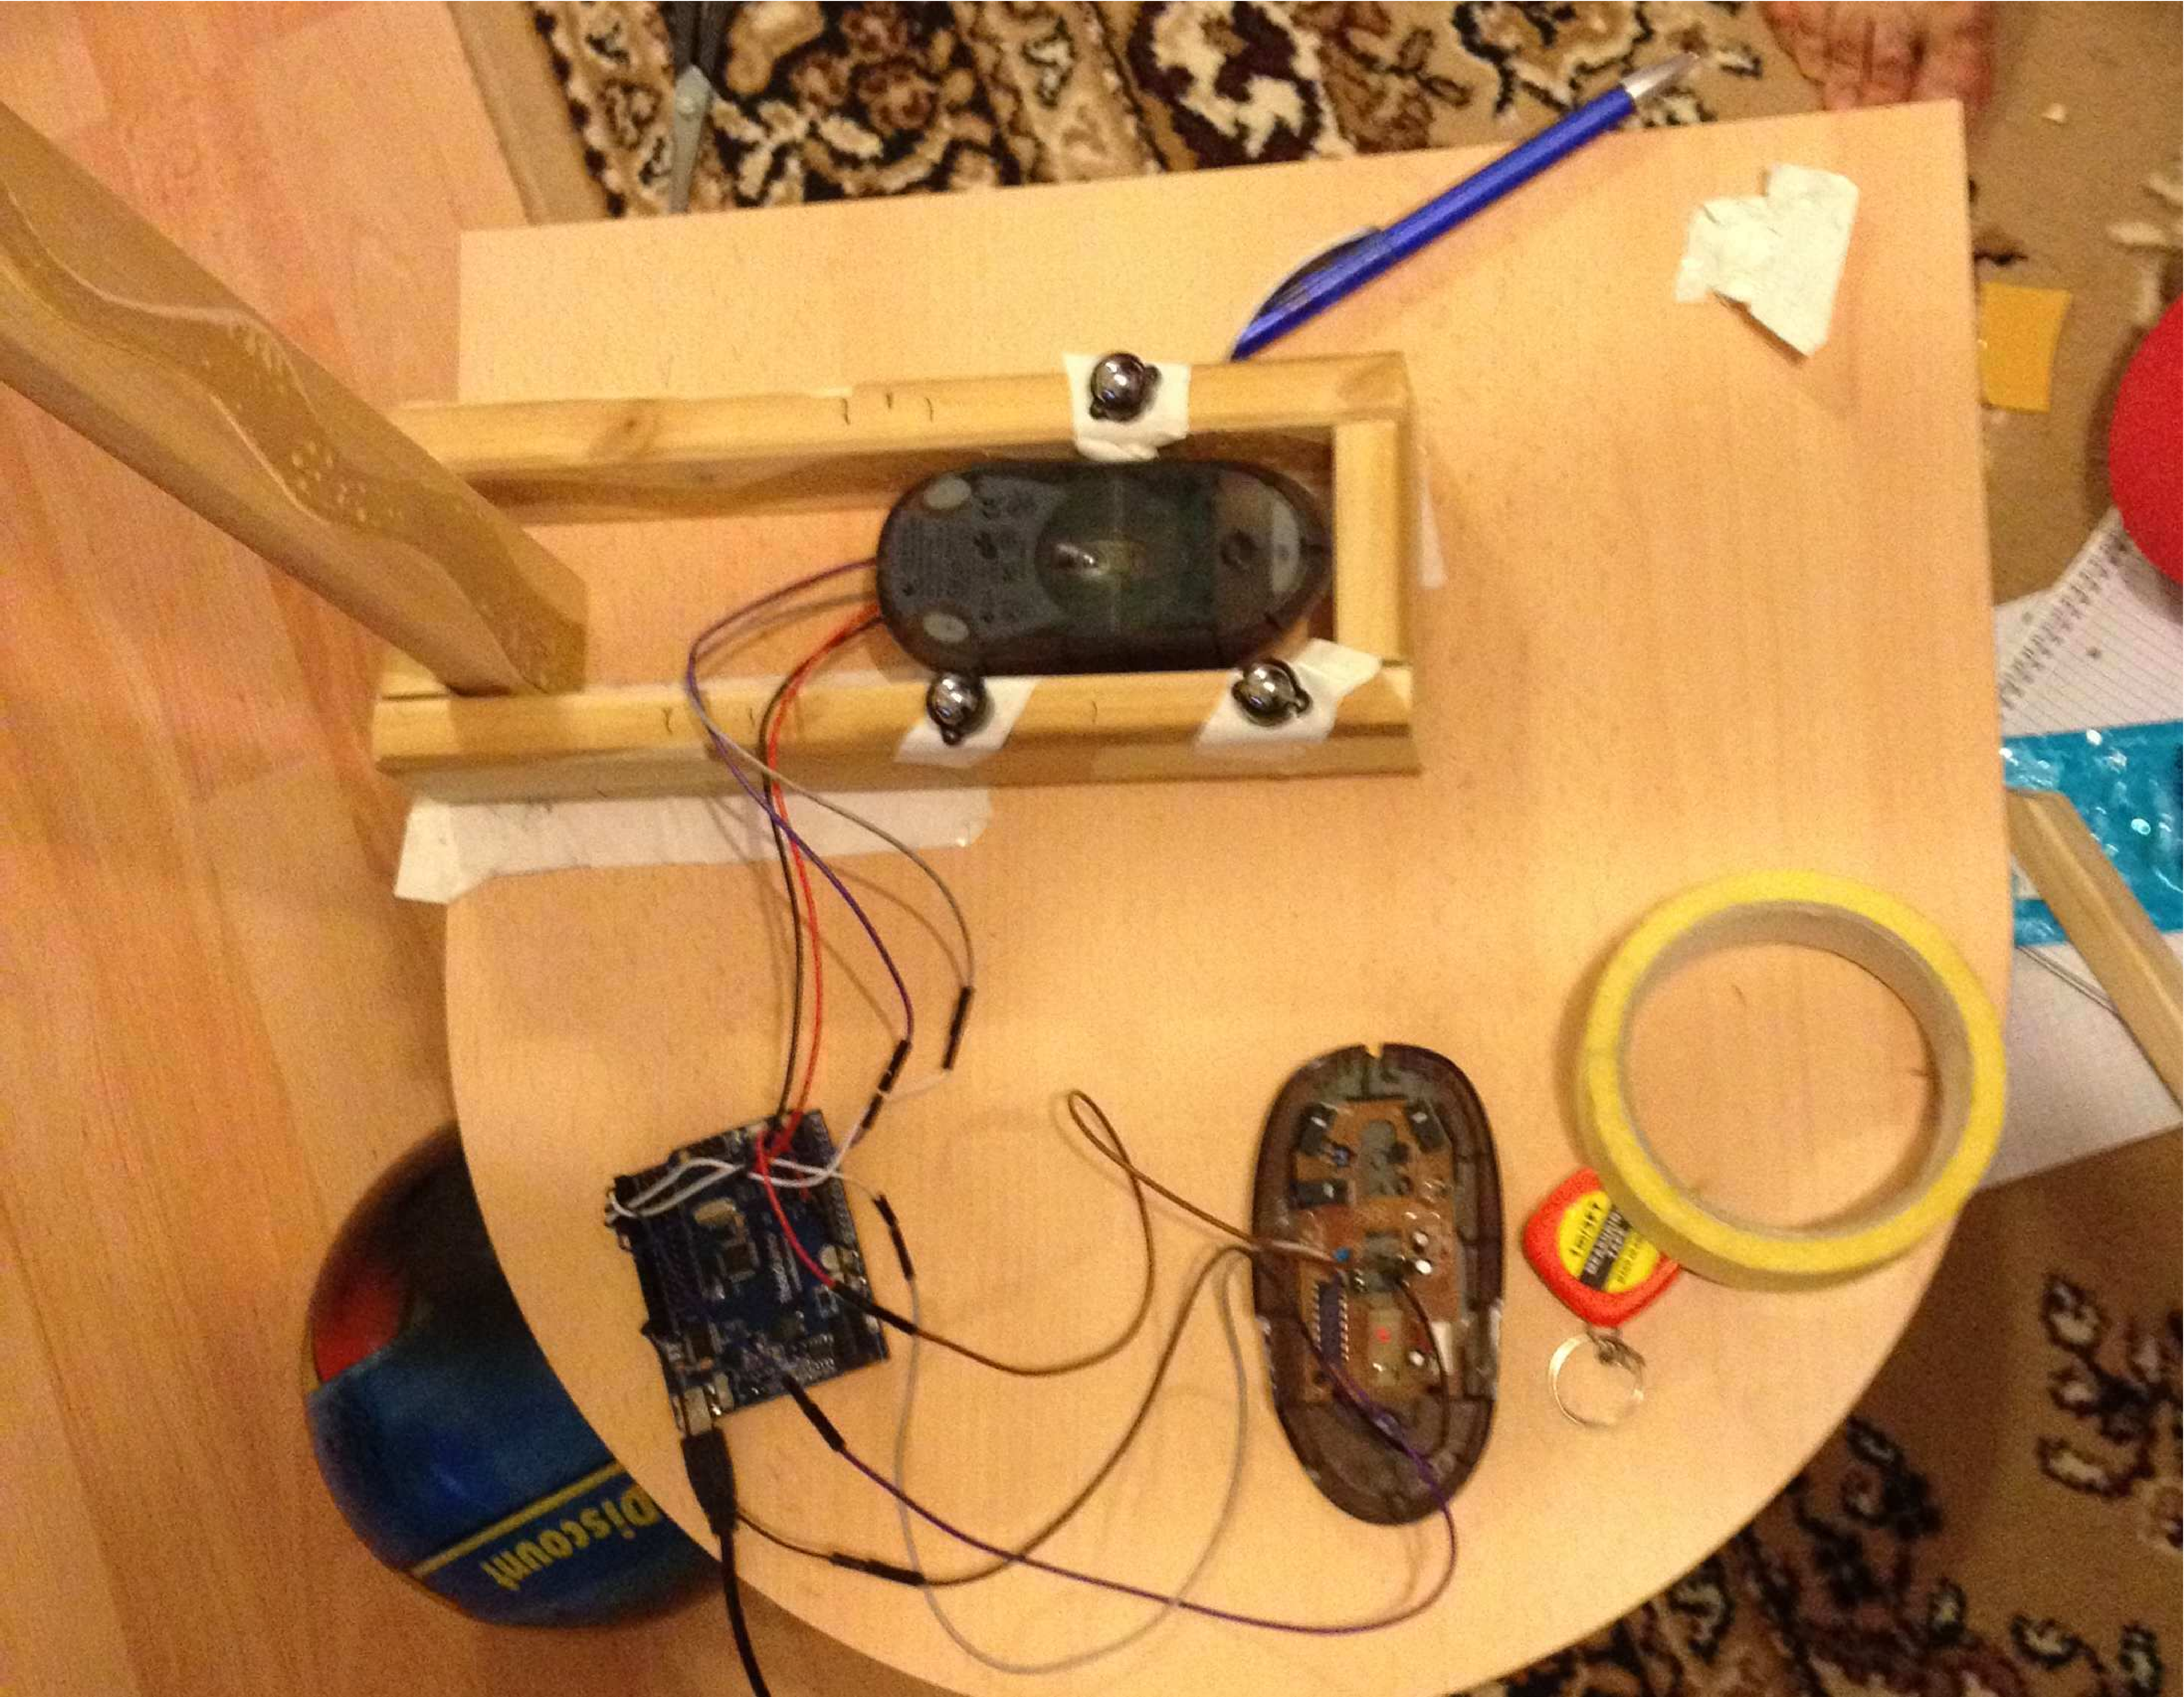
\includegraphics[scale=0.10]{prototype1-eps-converted-to.pdf} 
\caption{HCI Globe - 1st Sketch from above}\centering 
\label{fig:prot1}
\end{figure}	

\begin{figure}[ht!]\centering
%\includegraphics[scale=0.10]{prototype2.eps} 
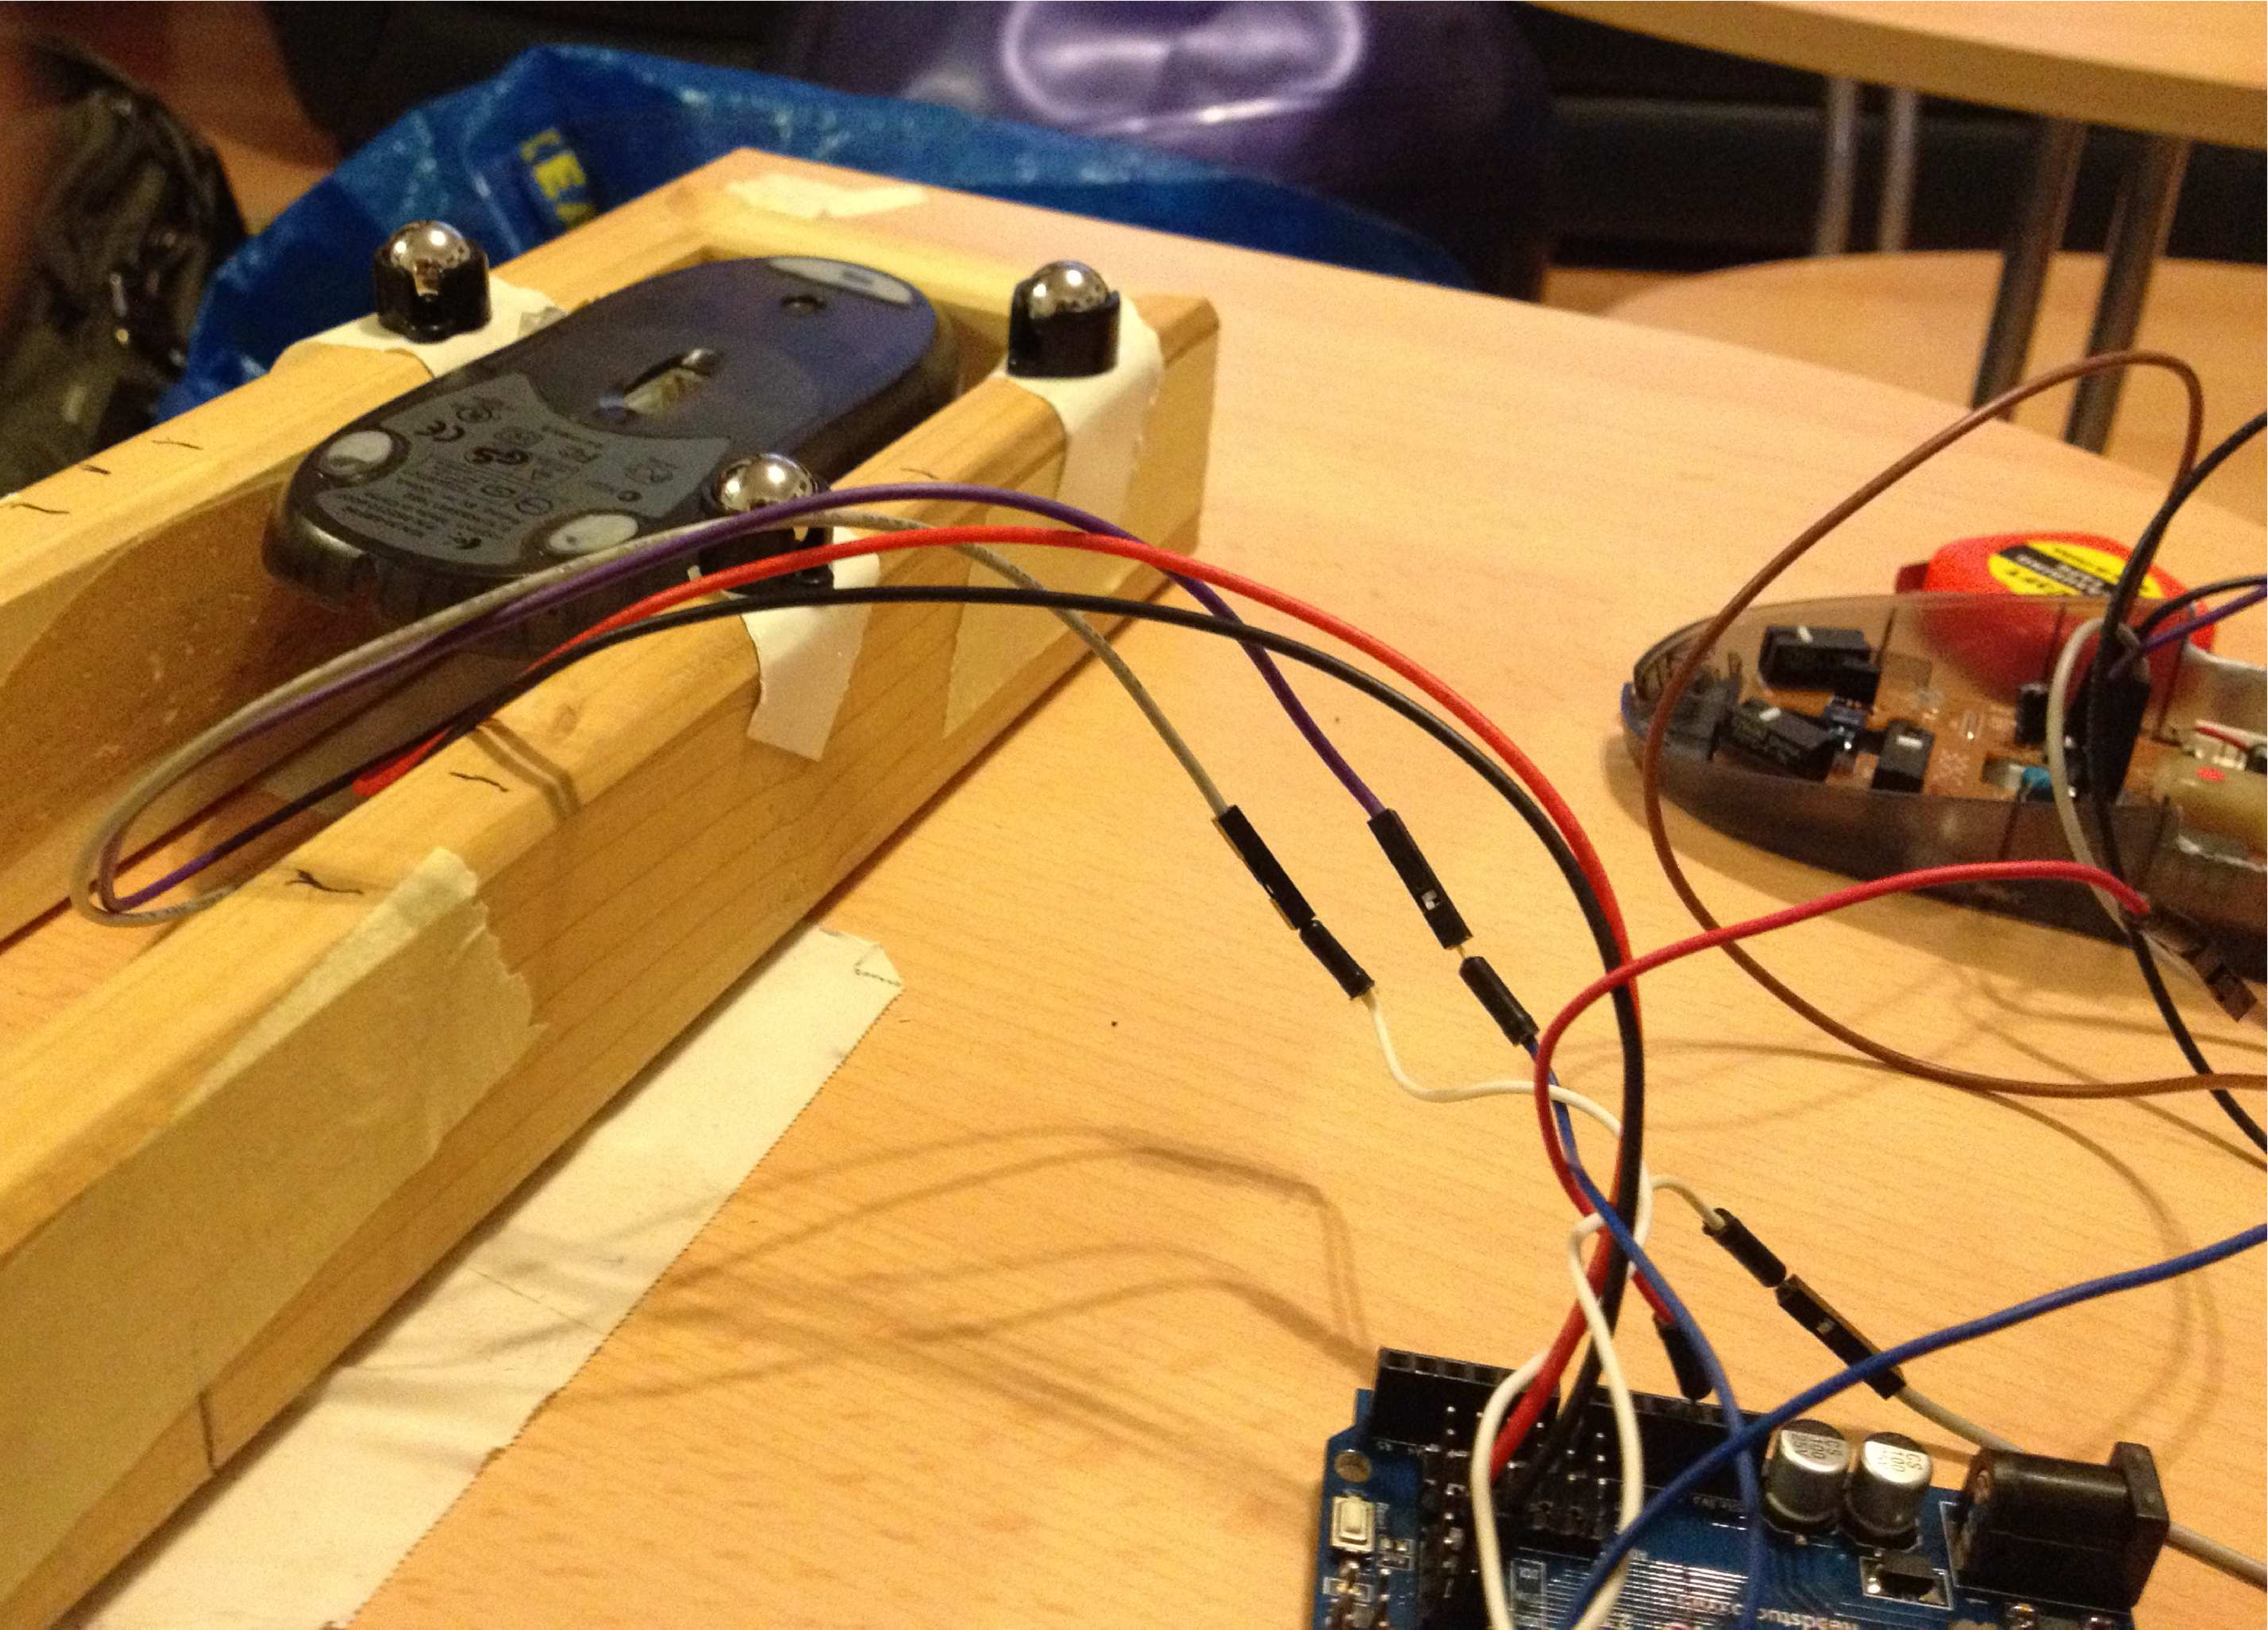
\includegraphics[scale=0.10]{prototype2-eps-converted-to.pdf} 
\caption{HCI Globe - 1st Sketch close up on the horizontal axis}\centering 
\label{fig:prot2}
\end{figure}	

In Figure \ref{fig:prot1} and Figure \ref{fig:prot2} it can be seen that only three caster balls were used for fixing the sphere in the vertical axis, but due to not satisfactory physical tests a fourth caster ball was introduced, making the sphere considerably more stable. Furthermore in the case development, the two mice were fixed using screws and a wooden stick was placed on top for better fixing of the rolling sphere, where later a fifth caster ball was placed. For giving a tidy look to the project, the Arduino board and the cables were placed inside the case, right between the two mice, as it can be seen in the Figure \ref{fig:prot4} and Figure \ref{fig:prot3}. 

\begin{figure}[ht]\centering
%\includegraphics[scale=0.085]{prototype4.eps} 
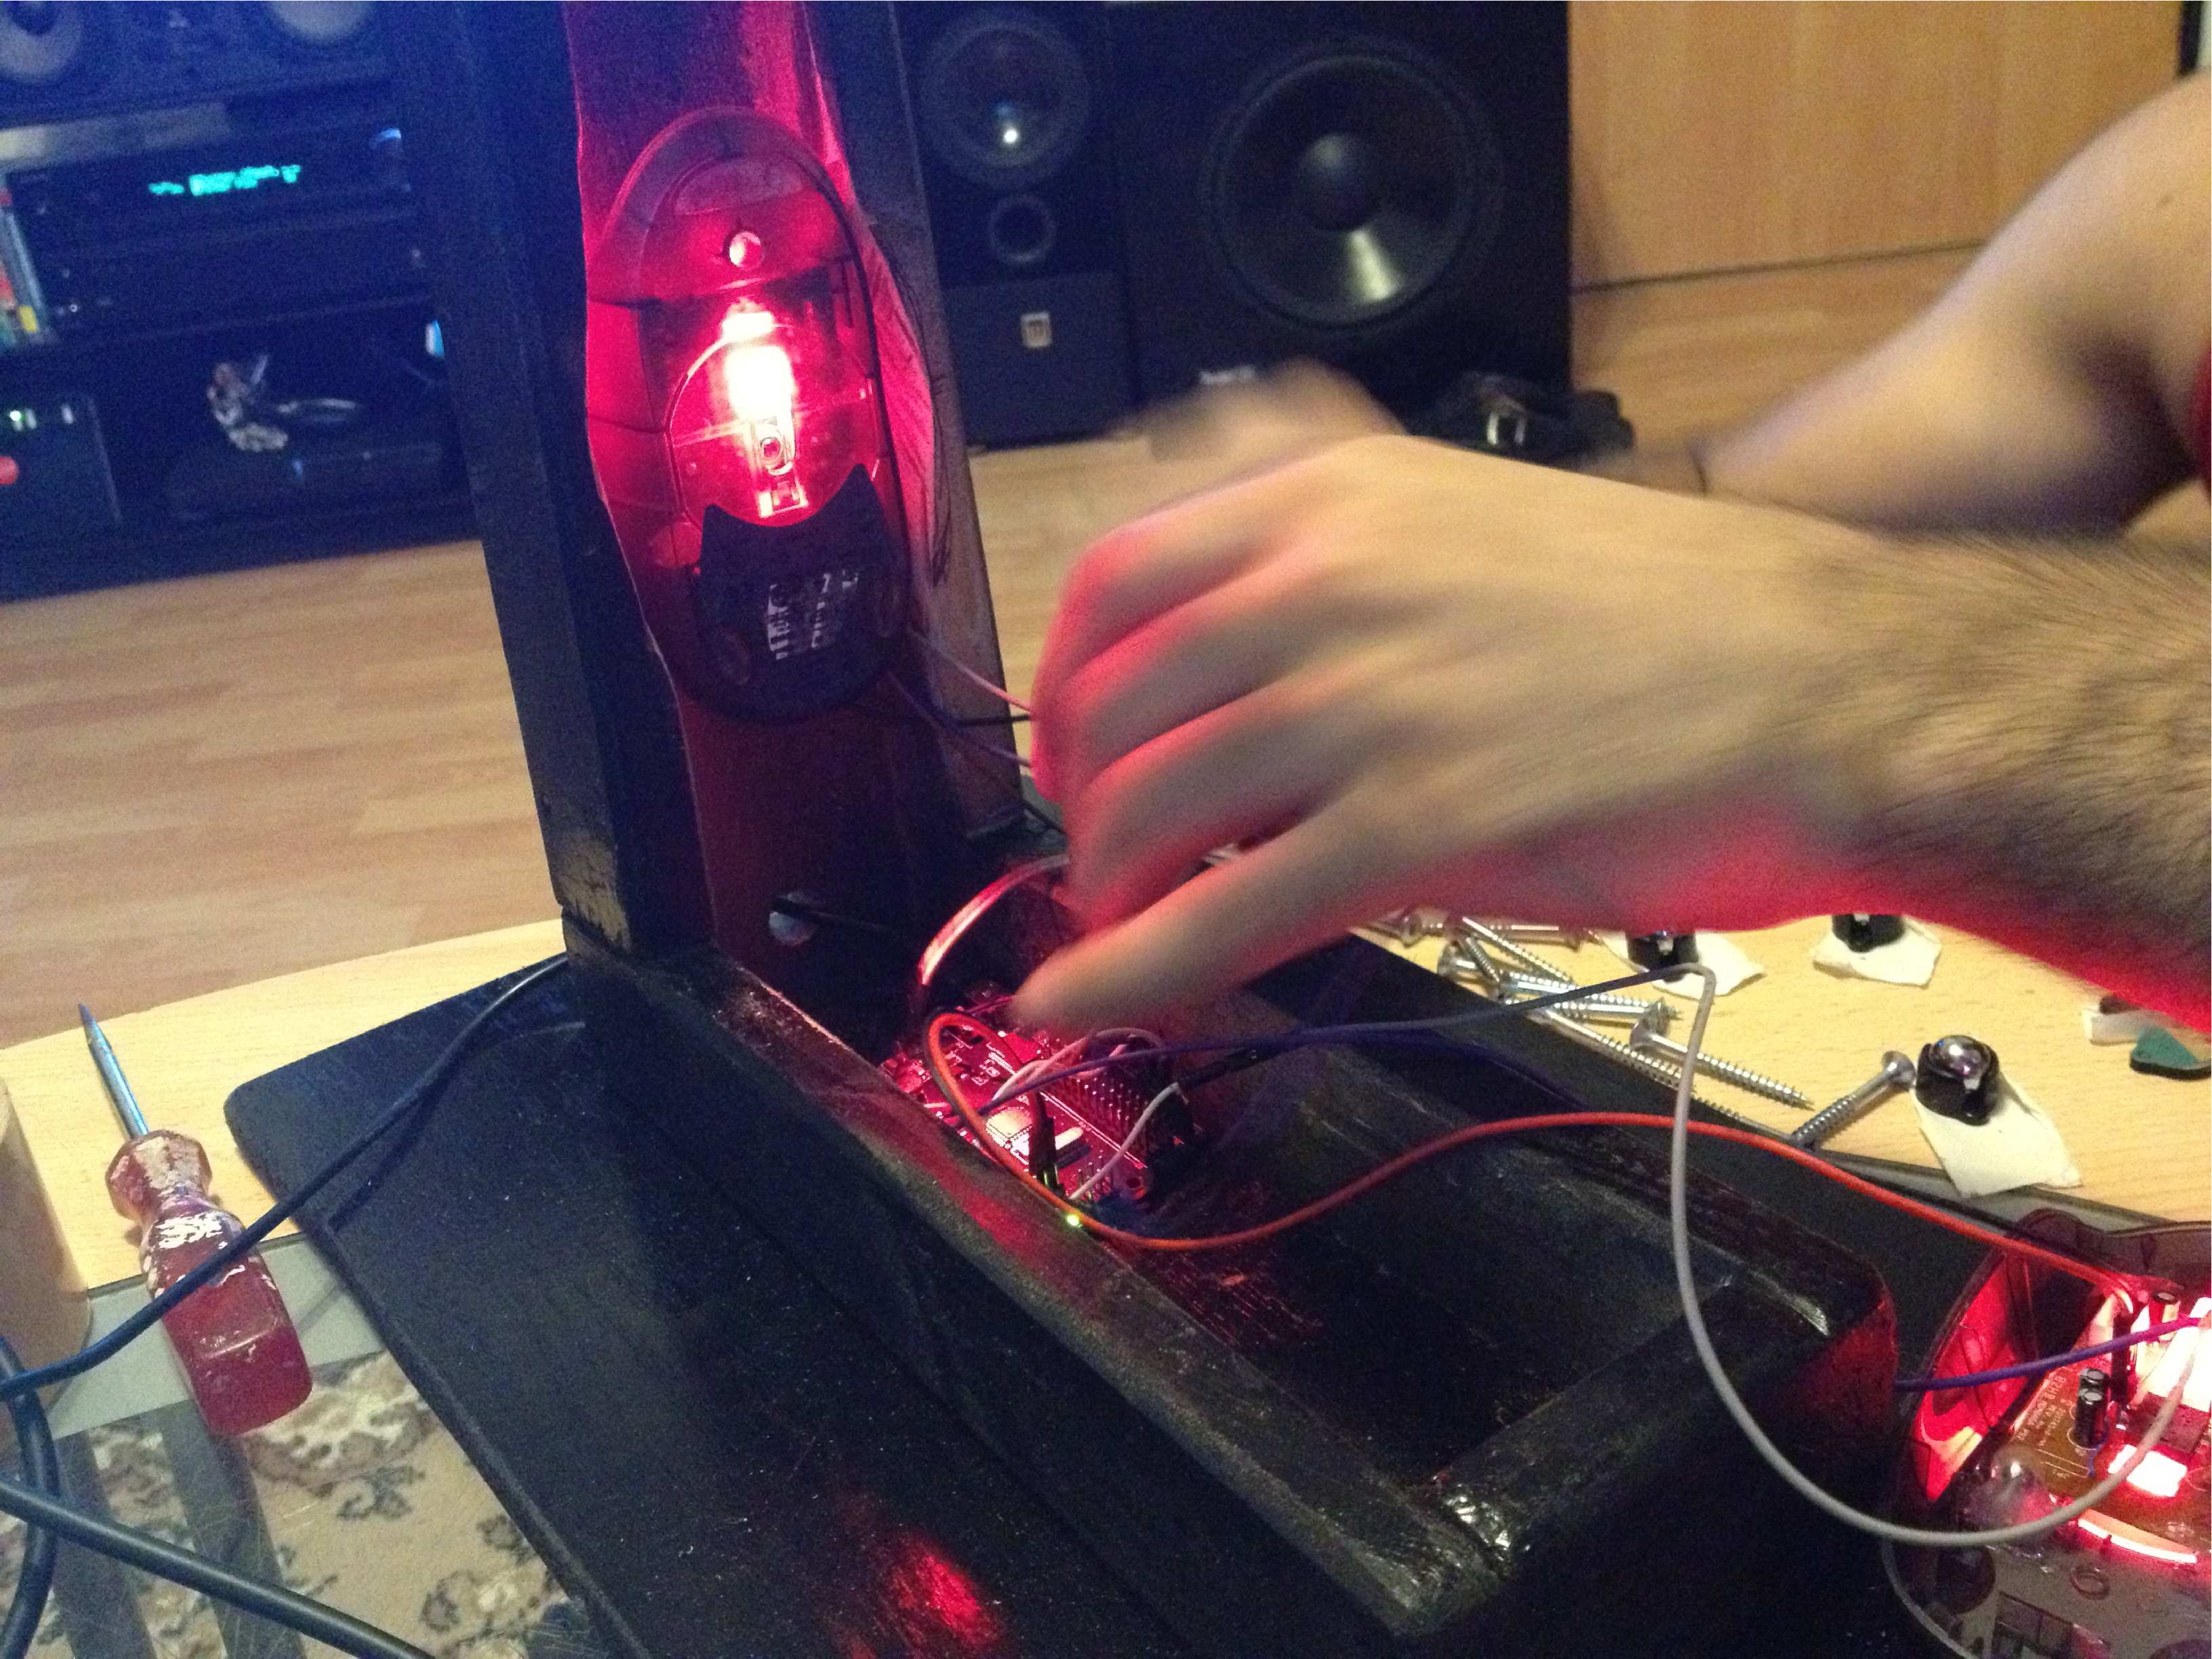
\includegraphics[scale=0.085]{prototype4-eps-converted-to.pdf} 
\caption{HCI Globe - Placing the mice and the Arduino board in the case}\centering 
\label{fig:prot4}
\end{figure}	

\begin{figure}[ht]\centering
%\includegraphics[scale=0.085]{prototype3.eps} 
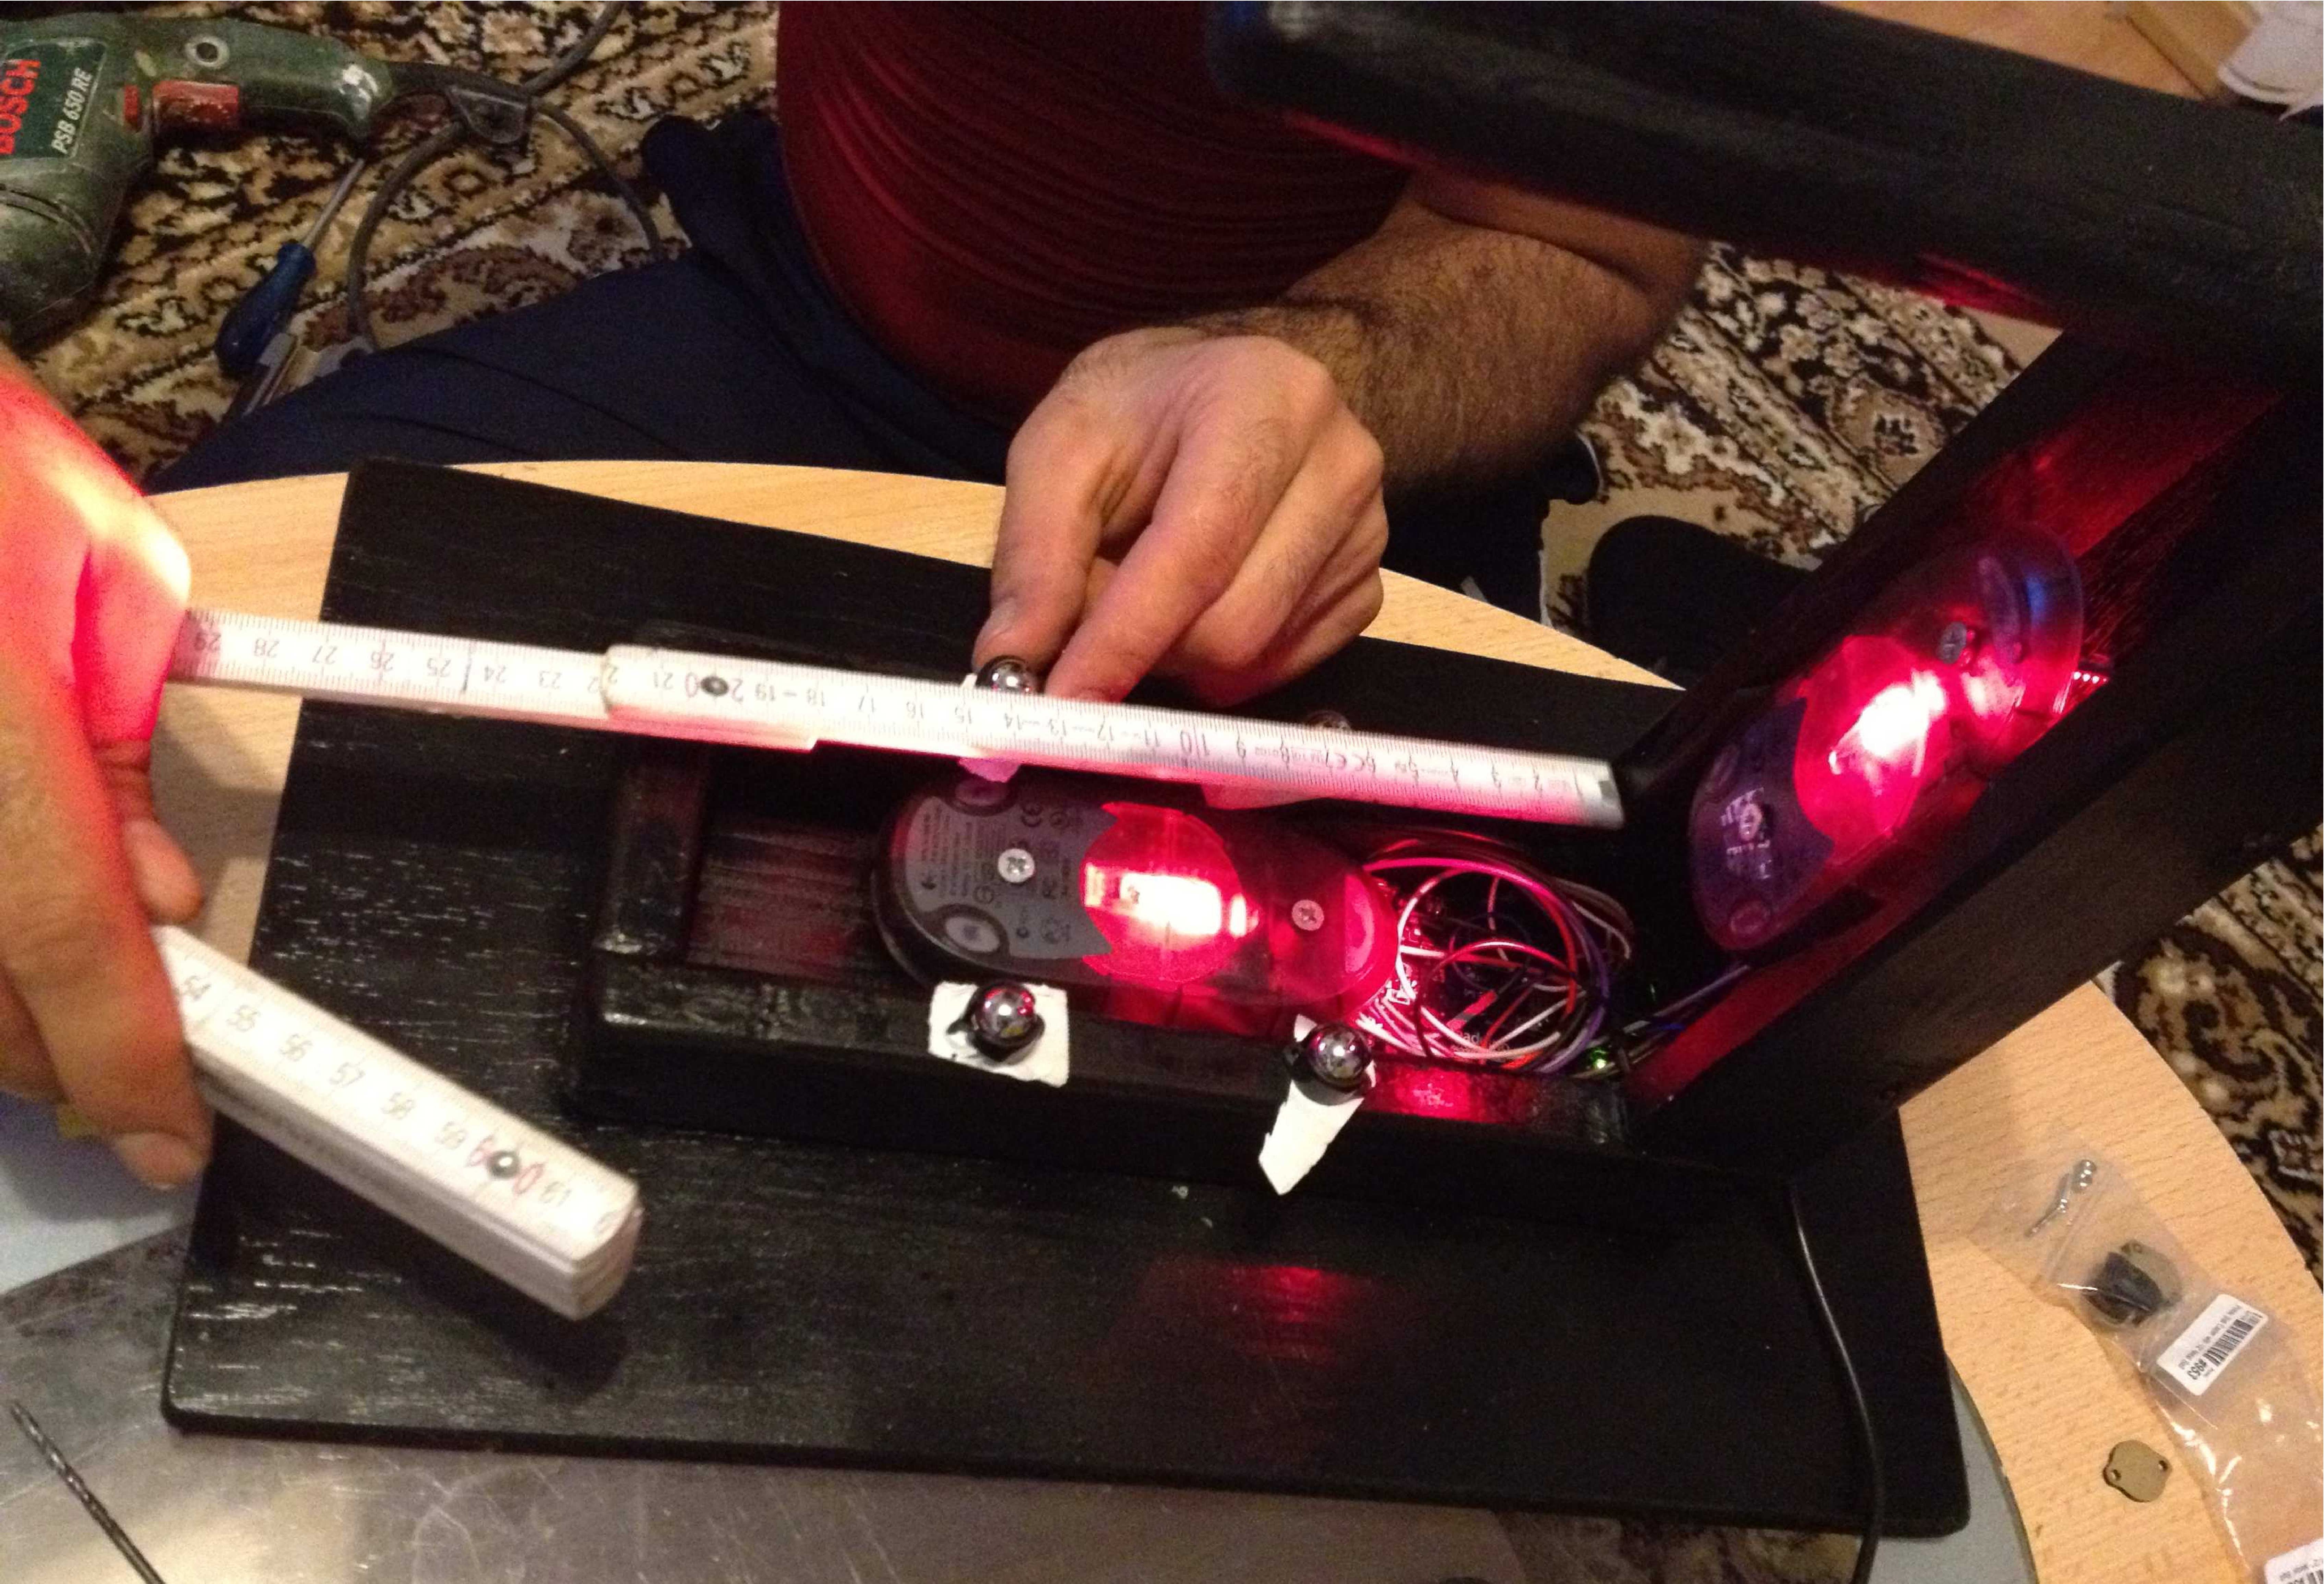
\includegraphics[scale=0.085]{prototype3-eps-converted-to.pdf} 
\caption{HCI Globe - Measuring the caster balls distance}\centering 
\label{fig:prot3}
\end{figure}	

The final version of the physical part of the project can be seen in the Figure \ref{fig:final}. A video with the HCI Terrestrial Globe presentation and usage can be found on YouTube under the title \textbf{Physical Computing - HCI Terrestrial Globe}\footnote{\url{http://www.youtube.com/watch?v=ryTRWwghDGQ}}.

\begin{figure}[ht]\centering
%\includegraphics[scale=0.10]{final.eps} 
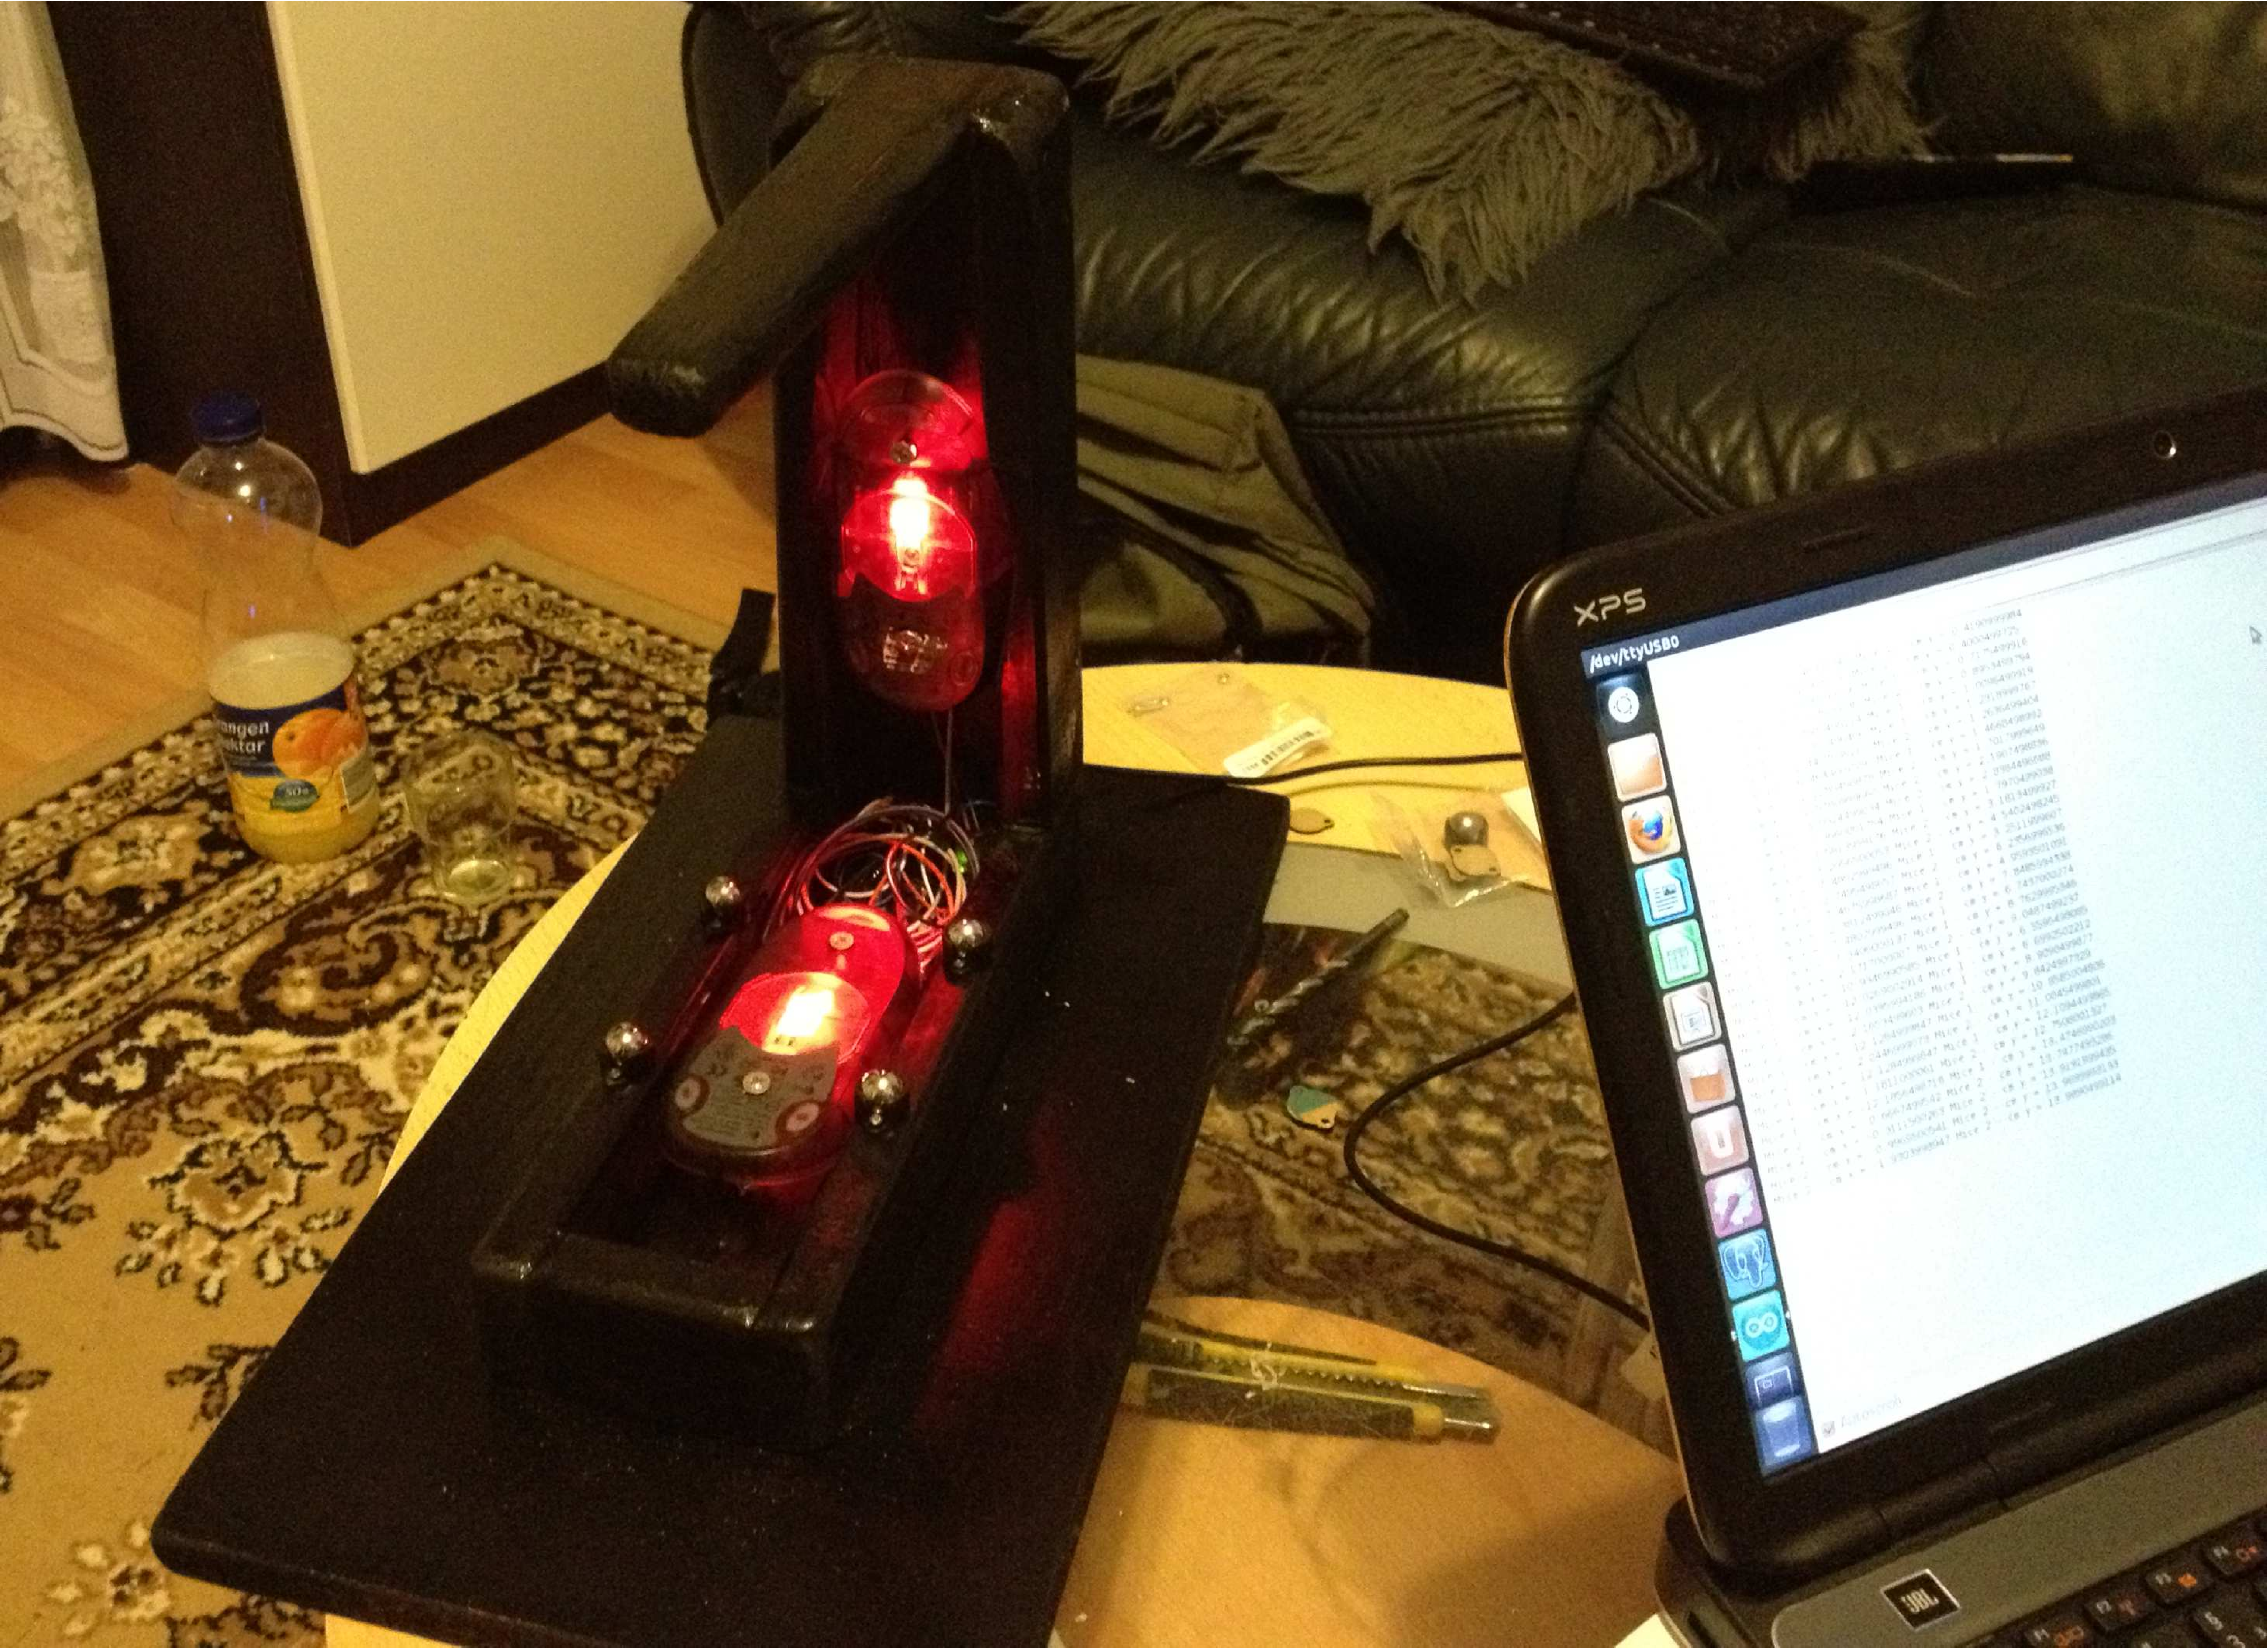
\includegraphics[scale=0.10]{final-eps-converted-to.pdf} 
\caption{HCI Globe - Final Version}\centering 
\label{fig:final}
\end{figure}	


\section{Arduino Embedded Software}

Once the physical part was done, the Arduino software was developed for acquiring direction and distance in the sphere movements. The optical sensor used in the project, the ADNS-2610, has a library \cite{martijn} that enables capturing movements performed using C code. This measurements are provided by the sensor / library using the unit CPI (Counts per Inch), which later we converted to the metric system, as it is well explained step by step in the code chunk bellow: 
\\
{
\scriptsize
\begin{verbatim}
#include "ADNS2610.h"

#define SCLK 2         // Serial clock pin on the Arduino - 1st mouse
#define SDIO 3         // Serial data (I/O) pin on the Arduino - 1st mouse
#define SCLK2 4        // Serial clock pin on the Arduino - 2nd mouse
#define SDIO2 5        // Serial data (I/O) pin on the Arduino - 2nd mouse

ADNS2610 Optical1 = ADNS2610(SCLK, SDIO); //1st mouse
ADNS2610 Optical2 = ADNS2610(SCLK2, SDIO2); //2nd mouse

double  x = 0;       // Variables for our 'cursor' 1st mouse
double  y = 0;       
double x2 = 0;       // Variables for our 'cursor' 2nd mouse
double y2 = 0;                        

int c = 0;          // Counter variable for coordinate reporting
double vX,vY,vX2,vY2 = 0; //Measurement variables for the mice

void setup()
{
  Serial.begin(38400); //Defining serial baud-rate
  Optical1.begin(); //Initializing 1st mouse                       
  Optical2.begin(); //Initializing 2nd mouse                    
}

void loop()
{
  x += Optical1.dx();   // Read the dX,dY register and in/decrease
  y += Optical1.dy();   // X,Y with that value for the 1st mouse.
  x2 += Optical2.dx();  // Read the dX,dY register and in/decrease
  y2 += Optical2.dy();  // X,Y with that value for the 2nd mouse.

  if ((x2 != vX2) || (y2 != vY2) || x != vX || y != vY) {
  //Only read if the current measurements are different as the last one,
  //to avoid unnecessary readings.
    if (c++ & 0x80){

    //Vertical mouse
      Serial.print(" M1_cm_x=");
      Serial.print(((x-vX)/400)*2.54, DEC);// Rotation in 3D-Z
      Serial.print(" M1_cm_y=");
      Serial.print(((y-vY)/400)*2.54, DEC);// Rotation in 3D-X
    //Horizontal mouse
      Serial.print(" M2_cm_x=");
      Serial.print(((x2-vX2)/400)*2.54, DEC);//  Rotation in 3D-Y
      Serial.print(" M2_cm_y=");
      Serial.print(((y2-vY2)/400)*2.54, DEC);//  Also 3D-X 

      c = 0;               // Reset the report counter
      Serial.println();     
    }
  }
  vX = x;
  vY = y;
  vX2 = x2;
  vY2 = y2;
}
\end{verbatim}
}

\section{Processing Software}

Processing\footnote{\url{http://processing.org}} is a programming language distributed as open source. For this project, and following the examples of Margolis \cite{Margolis}, it was used as client of serial communication messages sent by the Arduino board and transformed into computer's key-press events which are handled by the any active software at the moment. 

From the HCI terrestrial Globe, a received text message is parsed and transformed into numeric distance measurements over the rolling sphere. The Processing code takes care of achieving proportional movement among the rolling sphere and Google-Earth sphere through the \textit{rotatingTime} function which takes as parameters the rolling sphere's radius, the Eye Altitude (a parameter displayed on Google-Earth's user interface) and the distance measured by the HCI terrestrial Globe along a single axis. This function implements a statistical regression model derived from a set of observations and returns the duration of a click event on in order to match the movements of Google Earth  and the rolling sphere.

{
\scriptsize
\begin{verbatim}
import processing.serial.*;
import java.awt.Robot;
import java.awt.AWTException;
import java.awt.event.KeyEvent;

Serial myPort;      // Create object from Serial class
Robot myRobot;      // create object from Robot class;

public static final short LF = 10;
public static final short portIndex = 0;// select the com port, 0 is the first
int movCounter = 0;// Counter of the total number of movements made in Google Earth
float teddyBallRadiusCms = 10.1;//Radius of the small ball
float googleEarthEyeAltKms = 2999.28;//Google Eath's Eye Alt in Kms - see GE's lower right corner

void setup() {
    size(200, 200);
    println(Serial.list());
    println(" Connecting to -> " + Serial.list()[portIndex]);
    myPort = new Serial(this,Serial.list()[portIndex], 38400);    //Check the baudio values(i.e 9600)
    try {
        myRobot = new Robot(); // the Robot class gives access to the mouse
    }catch (AWTException e) { // this is the Java exception handler
        e.printStackTrace();
    }
}

void draw() {
}

void serialEvent(Serial p) throws InterruptedException{
    String message = myPort.readStringUntil(LF); // read serial data
    if(message != null){
        message = message.trim();// Whitespace removal
        String [] data = message.split("\\s+"); // Split the whitespace-separated message
        //Get the tag-value pairs
        String m1xStr = data[0].trim();
        String m1yStr = data[1].trim();
        String m2xStr = data[2].trim();
        String m2yStr = data[3].trim();
        //Splits the tag-value pairs
        String [] m1x = m1xStr.split("=");
        String [] m1y = m1yStr.split("=");
        String [] m2x = m2xStr.split("=");
        String [] m2y = m2yStr.split("=");
        //Gets the values
        float x1 = float(m1x[1]);
        float y1 = float(m1y[1]);
        float x2 = float(m2x[1]);
        float y2 = float(m2y[1]);

        int sleep = 0;

        //3D-Z
        if(x1 > 0){
            myRobot.keyPress(KeyEvent.VK_LEFT);
            //Time estimation of how long the key should be pressed
            sleep = rotatingTime(googleEarthEyeAltKms, teddyBallRadiusCms, x1);
            Thread.sleep(sleep);
            myRobot.keyRelease(KeyEvent.VK_LEFT);
            movCounter++;
            println(movCounter + " Rotating Z -> " + sleep);
        }else if(x1 < 0){
            myRobot.keyPress(KeyEvent.VK_RIGHT); 
            sleep = rotatingTime(googleEarthEyeAltKms, teddyBallRadiusCms, x1);
            Thread.sleep(sleep);
            myRobot.keyRelease(KeyEvent.VK_RIGHT); 
            movCounter++;
            println(movCounter + " Rotating Z <- " + sleep);
        }

        //3D-X
        if(y1 > 0){
            myRobot.keyPress(KeyEvent.VK_UP);
            sleep = rotatingTime(googleEarthEyeAltKms, teddyBallRadiusCms, y1);
            Thread.sleep(sleep);
            myRobot.keyRelease(KeyEvent.VK_UP);
            movCounter++;
            println(movCounter + " Rotating X v " + sleep);
        }else if(y1 < 0){
            myRobot.keyPress(KeyEvent.VK_DOWN);
            sleep = rotatingTime(googleEarthEyeAltKms, teddyBallRadiusCms, y1);
            Thread.sleep(sleep);
            myRobot.keyRelease(KeyEvent.VK_DOWN);
            movCounter++;
            println(movCounter + " Rotating X ^ " + sleep);
        }

        //3D-Y
        if(x2 > 0){
            myRobot.keyPress(KeyEvent.VK_SHIFT);
            myRobot.keyPress(KeyEvent.VK_LEFT);
            sleep = rotatingTime(googleEarthEyeAltKms, teddyBallRadiusCms, x2);            
            Thread.sleep(sleep);
            myRobot.keyRelease(KeyEvent.VK_SHIFT);
            myRobot.keyRelease(KeyEvent.VK_LEFT); 
            movCounter++;
            println(movCounter + " Rotating Y -v " + sleep);
        }else if(x2 < 0){            
            myRobot.keyPress(KeyEvent.VK_SHIFT);
            myRobot.keyPress(KeyEvent.VK_RIGHT); 
            sleep = rotatingTime(googleEarthEyeAltKms, teddyBallRadiusCms, x2);            
            Thread.sleep(sleep);
            myRobot.keyRelease(KeyEvent.VK_SHIFT);
            myRobot.keyRelease(KeyEvent.VK_RIGHT); 
            movCounter++;
            println(movCounter + " Rotating Y -^ " + sleep);            
        }
    }
}

//This function estimates the duration the KEY PRESS event to sync balls movements
int rotatingTime(float googleEarthEyeAltKms, float teddyBallRadiusCms, float teddyBallDistanceCms){

  float geEyeAlt = googleEarthEyeAltKms;//Google Eath's Eye Alt in Kms - see GE's lower right corner
  float tBallR = teddyBallRadiusCms;// Radius of the Teddy Ball in cms
  float tBallD = abs(teddyBallDistanceCms);//Distance over Teddy Ball's surface in cms
  float tBallP = 2 * PI * tBallR;//TBall perimeter
  float tBallA = tBallD * 360 / tBallP;//tBall surface distance as an angle (in degrees)
  float geCompleteTurn = (-4.841 * log(geEyeAlt)) + 58.222;// Time (seconds) for a complete turn of google earth
  float t = tBallA *geCompleteTurn / 360;// Key pres time (secs) for moving GE in the same angle as tBall
  t = t * 1000;// Secs to millisecs * 1000
  int res = (int)(t*100);// Little adjustment *100
  return res;
}
\end{verbatim}
}

%\section{Conclusion}

\begin{thebibliography}{6}

\bibitem{Margolis}
Arduino Cookbook, Recipes to begin, Expand, and Enhance your Projects, 2006\\
Michael Margolis\\

\bibitem{martijn}
Interfacing an optical mouse sensor to your Arduino, 2008\\
Martijn Th\'e\\
\scriptsize\url{http://www.martijnthe.nl/2009/07/interfacing-an-optical-mouse-sensor-to-your-arduino/}\\
 

\end{thebibliography}

\bibliographystyle{abbrv}
\bibliography{main}


\end{document}
